% !TeX spellcheck = es_ES
% !TeX program = pdflatex
\documentclass[twocolumn,11pt]{article}

\usepackage[utf8x]{inputenc}
\usepackage[spanish]{babel}
% Hyperref antes de geometry
\usepackage[
hyperfootnotes=false,
urlcolor=blue,
colorlinks=true,
citecolor=red,
linkcolor=blue]{hyperref}

\usepackage[a4paper,top=2.5cm,bottom=2cm,left=1.65cm,right=1.65cm,marginparwidth=1.75cm,headheight=28pt]{geometry}
\setlength{\columnsep}{.8cm}
%Letra general
\usepackage{mathastext}

\renewcommand{\familydefault}{\sfdefault}
%\usepackage[scaled=1]{helvet}
\usepackage[format=plain,
            labelfont={bf,it},
            textfont=it]{caption}
            
\usepackage{xcolor}

\usepackage{fontawesome}
\usepackage{siunitx}
\usepackage{graphicx}
%Math
\usepackage{amsmath,amssymb}
\usepackage{amsfonts}
\usepackage{fancyhdr,framed}
\setlength{\headheight}{22.5pt}
\pagestyle{fancy}
\lhead{\href{http://www.whittileaks.com}{\textsf{whittileaks.com}}}
\chead{MCI}

%commands
\newcommand{\glossentry}[2]{$#1$\indent #2 \par \vspace{.4cm} } %Entradas para glosario
\newcommand{\agma}{\textrm{AGMA }}
\newcommand{\bigpar}[1]{\bigg(
#1 \bigg) }
\newcommand{\dprime}{ {\prime \prime} }
\newcommand{\di}{\textrm{d}}
\newcommand{\tprime}{ {\prime \prime \prime} }
\newcommand{\fit}{\textit{\textrm{f }}}
\newcommand{\corr}{{\textrm{\color{red} Revisar}}}
\newcommand{\Kf}[1]{ K_{\textit{\textrm{f}}_{\textrm{#1}}} }
\newcommand{\Kfs}[1]{ K_{\textit{\textrm{fs}}_{\textrm{#1}}} }
\newcommand{\siga}[1]{ \sigma_{{\textrm{a}}_{\textrm{#1}}} }
\newcommand{\sigm}[1]{ \sigma_{{\textrm{m}}_{\textrm{#1}}} }
\newcommand{\pe}{\textit{\textrm{p}}}
\newcommand{\gut}{{\color{green}\faCheck}}
\newcommand{\HC}{$H_xC_y$}
\newcommand{\NX}{$NO_x$}
\begin{document}
\title{Resumen de Motores a Combustión interna}


% \author{Carlos Oncha}
% \maketitle
\onecolumn[
\centering 
{\bf \huge Resumen de Motores a Combustión Interna \par}
\vspace{.2cm}
{\sc \large El Chispero\par }
\vspace{.4cm}\par
\tableofcontents
]
\twocolumn{
\newcommand{\rc}{R_c}
\newcommand{\Calorif}{\mbox{\large$\mathbf{c}$}}
\newcommand{\rp}{R_p}
\newcommand{\grad}{$^\circ$}
\newcommand{\Fp}{F_P}
\newcommand{\Peff}{P}
\newcommand{\ideal}{{ideal}}
\newcommand{\perd}{{perd.}}
\newcommand{\Pideal}{P_\ideal}
\newcommand{\Pperd}{P_\perd}
\newcommand{\Pind}{P_i}
\newcommand{\pmi}{p_{mi}}
\newcommand{\Pot}{{ \mbox{\tiny$P$}}}
\newcommand{\Potmax}{{ \mbox{\tiny$P_\max$}}}
\newcommand{\Torq}{{ \mbox{\tiny$T$}}}
\newcommand{\Torqmax}{{ \mbox{\tiny$T_\max$}}}
\newcommand{\Ce}{C_e}
\newcommand{\pme}{p_{me}}
\newcommand{\etaeff}{\eta_{total}}
\newcommand{\etavol}{\eta_{{\mbox{\tiny$V$}}}}
\newcommand{\util}{\acute{u}til}

\renewcommand{\min}{{m\textrm{í}n}}
\renewcommand{\max}{{m\acute{a}x}}
\newcommand{\ctegas}{k}
\newcommand{\rv}{{R_{\mbox{\tiny $V$}}}}
 \mathchardef\mhyphen="2D
 \newcommand{\hyph}{\,\mhyphen}
 \vspace{.9cm}
{\centering 
{\bf \LARGE Primer Parcial \par}
}
\begin{center}
\vspace{-.2cm}\rule{3cm}{2pt}\par
\vspace{-.2cm}
\end{center}

\section{Que son estas cosas?}

Un motor térmico es cualquier dispositivo que puede quemar una mezcla de aire y combustible en una cámara de combustión (interna o externa) y convertir dicha energía térmica en energía mecánica.

\begin{itemize}
    \item {\bf Motores a combustión interna o endotérmicos:} El cambio térmico se genera en el mismo fluido de trabajo en el interior del motor.
    \item {\bf Motores de combustión externa o exotérmicos:} Al fluido de trabajo se le transmite el estado térmico a través de una pared (como una turbina).
    \begin{itemize}
        \item Fueron usados extensivamente durante la revolución industrial.
        \item Rendimiento bajo y alta contaminación.
    \end{itemize}
\end{itemize}

Tipo de motor endotérmico (MCI):
\begin{itemize}
    \item \textbf{MEP}: Motores de encendido provocado.
    \item \textbf{MEC}: Motores de encendido por compresión.
\end{itemize}

Motores ciclo Otto son encendidos a chispa mientras que los motores a ciclo Diesel se encienden por compresión. La diferencia principal entre estos motores es que el calor aportado en el Otto idealizado ocurre a volumen constante (en un instante) mientras que en el Diesel el calor es aportado a volumen constante.
% \begin{itemize}

    
% \end{itemize}
{\bf Potencia en motores.} Si quiero más potencia en un \textbf{Otto} entrego más \textit{aire y combustible}. Si quiero hacer lo mismo en un \textbf{Diesel} entrego más \textit{combustible}. La eficiencia térmica en motores está dada por:

\[
\eta_t=\frac{W_{\util}}{Q_{entregado}}=\frac{Q_{entregado}-Q_{perdido}}{Q_{entregado}}=1-\frac{Q_{perd}}{Q_{entr}}
\]
Para un Otto esto vale:
\[
\eta_{t_{Otto}}=1-\frac{1}{\ctegas}\frac{T_4-T_1}{T_3-T_2}
\]
\subsection{Otto en pequeños detalles}

\textbf{El combustible nafta o gasolina.} 
\begin{itemize}
    \item Mezcla pobre es preferible por razones de contaminación 
    \item Mezcla estequiométrica:\textit{Aire a gasolina} \textbf{14,7:1} (masa) 
    \begin{itemize}
        \item Reducir esta relación (mezcla más rica) aumenta contaminación y crea humo negro (material particulado) y otros problemas
    \end{itemize}
    \item Densidad \textbf{0,71-0,76 kg/lt} con un poder calorífico de $\Calorif_{nafta}\cong$ \textbf{44.000 kJ/kg}
\end{itemize}

\textbf{Características del motor Otto.}
\begin{itemize}
\item Encendido logrado con un arco eléctrico con bujías
\item Inyector de combustible puede estár dentro de la conjunto pistón o en el trayecto de admisión. (Diesel solo adentro)
\item Mayor contenido de $CO$ monoxido de carbono en los gases de escape comparado al Diesel.
\item Presiones menores a las del Diesel en general
\item Comparado a Diesel grado de compresión bajo. $\rc = 8\,\mhyphen 11$ con presión $p_{compresi\acute{o}n}=13\,\mhyphen15\, bar$ y $p_\max=30\,\mhyphen40\,bar$.
\end{itemize}
{\bf Diagrama del ciclo Otto 4 tiempos.}
\begin{itemize}
    \item {\bf Admisión}
    \begin{itemize}
        \item El pistón desciende desde el PMS al PMI. Válvula de admisión abierta y la de escape cerrada
    \end{itemize}
    \item \textbf{Compresión}
    \begin{itemize}
        \item Se cierra la válvula de admisión y sube el pistón al PMS. $p_f=10-15\,bar$
    \end{itemize}
    \item  \textbf{Expansión}
    \begin{itemize}
        \item Se produce la chispa y por ende la combustión antes del PMS. Durante la expansión el pistón desciende del PMS al PMI produciéndose el trabajo útil
    \end{itemize}
    \item \textbf{Escape}
    \begin{itemize}
        \item El pistón sube del PMI al PMS con la válvula de escape abierta extrayéndose los gases de combustión
        \item El ciclo se vuelve a repetir en estos 4 pasos
    \end{itemize}
\end{itemize}

ESTUDIAR CICLOS.

Seguimos en \textbf{OTTO.}
\begin{itemize}
    \item \textbf{AAA:} Avance a la apertura de la válvula de admisión
    \item \textbf{AAE:} Avance a la apertura de la válvula de escape
    \item \textbf{RCE:} Retraso al cierre de la válvula de escape
    \item \textbf{RCA:} Retraso al cierre de la válvula de admisión
    \item \textbf{AE:} Avance de encendido
    \begin{itemize}
        \item Varía entre $5^\circ-40^\circ$
    \end{itemize}
    \item \textbf{CV=AAA+RCE:} Cruce de válvulas
\end{itemize}

\subsection{Volumen de cilindro}
Se tiene el volumen unitario $V_u$, definido como el volumen que ``barre'' el pistón en su recorrido. El volumen de cámara de combustión es el volumen \textit{mínimo} alcanzado durante la combustión. $V$ es el volumen total o cilindrada, equivalente al volumen unitario multiplicado por cantidad de cilindros: $V=V_u\cdot N$

\[
\rc=\frac{V_u+V_c}{V_c}
\]
$\rc$ es la relación de compresión del motor la cual define varias eficiencias.

Si se considera el gas de la cámara como ideal se puede definir el \textbf{rendimiento térmico del Otto} como

\[
\eta_t=1-\frac{1}{\rc^{\ctegas-1}}=1-\left(\frac{V_\min}{V_\max}\right)^{\ctegas-1}
\]
donde $\ctegas=\frac{c_p}{c_v}\approx1,33$ para Otto.

\textbf{Cruce de válvulas.} Se produce con la apertura simultanea de las válvulas de admisión y escape al fin de la etapa del escape. Esto permite que aún con el pistón detenido en el PMS los gases circulen gracias a su inercia térmica, trayendo aire fresco. Esto refrigera el cilindro y aumenta la concentración de aire para el próximo ciclo.

A medida que aumenta el número de vueltas (la velocidad [rpm del cigüeñal]) el tiempo de intercambio de gases se reduce. Por lo tanto se necesita aumentar el cruce de válvulas. Cuanto más rápido el motor$\Rightarrow$ Mayor cruce de válvula. Para motores Otto $CV=0-35^\circ$

\subsection{Motor Diesel en detalles chicos}

\textbf{El combustible diesel o gasóleo.} 
\begin{itemize}
    \item Siempre funciona a exceso de aire. 
    \item Mezcla estequiométrica: \textit{Aire a gasóleo} \textbf{14,5:1} (masa)
    \begin{itemize}
        \item Reducir esta relación (mezcla más rica) aumenta contaminación y crea humo negro (material particulado) y otros problemas
    \end{itemize}
    \item Densidad \textbf{0,81-0,85 kg/lt a }$15^\circ C$ con un poder calorífico de $\Calorif_{Diesel}\cong$ \textbf{42.000 kJ/kg}
    \item Viscosidad aumenta violentamente con descenso de temperatura. Se necesita un precalentador para $T\approx-25^\circ$
\end{itemize}
Como bien se menciono anteriormente, la potencia es otorgada por un aumento de combustible, \textit{no hay cambio de cantidad de aire en la cámara}. Al acelerar se aumenta la cantidad de combustible y aumenta la potencia erogada por el motor.

\textbf{Método de inyección.}
Dos métodos principales para motores Diesel:
\begin{itemize}
    \item Motores de inyección directa (a la cámara de combustión)
    \begin{itemize}
        \item Mejor rendimiento térmico y especifico
        \item Requiere biela y cigüeñal robustos
        \item 99,9\% motores de este tipo
    \end{itemize}
    \item Motores de inyección ``indirecta'' lo hacen en una precámara de inyección
    \begin{itemize}
        \item Vibraciones mas suaves, mejor para autos pequeños
        \item Contamina más
    \end{itemize}
\end{itemize}

\textbf{Características de la preinyección en el Diesel.} Para motores chicos se efectúa una o multiples pre-inyecciones que con el tiempo llegan a homogenizarse en la cámara completamente y luego se enciende \textit{antes} de la inyección principal. Con esto se logra que la inyección principal caiga sobre un frente de llama, acelerando el proceso de combustión. Dicho esto, el retraso de tiempo de ignición se achica considerablemente.

{\bf Características del motor Diesel.}
\begin{itemize}
    \item No existe mariposa de aceleración
    \item Exceso de aire es deseable
    \item Encendido al estar en contacto con aire a temperatura $T>500^\circ \,C$
    \item Aumento de temperatura de aire del ambiente afecta rendimiento negativamente\footnote{A mayor temperatura, menor densidad de aire $\Rightarrow$ menor masa de aire en cámara.}
    \item Bujías de \emph{precalentamiento}. Favorece arranque en frió
    \item Presiones mayores que en Otto. Componentes (biela, perno de pistón cigüeñal) reforzados
    \item Motores Diesel modernos en el rango de $\rc\approx 21$ y presión de combustión $p_{\max}\approx 190\,bar$, presión media efectiva $\pme\approx 25\, bar$ y presión de inyección (Common rail 3rd gen) $p_{iny}=2000\,\mhyphen 3000\, bar$
    \item \textbf{Diesel Lento:}Funcionamiento duro y ruidoso con alto tiempo de retraso. Inyectores de multiples orificios
    \item \textbf{Diesel Rápido:} Superan los 4500 rpm. Común usar camaras combustión integradas al pistón. Preinyecciones (3-10\% de inyección total) antes de inyección principal (ayudan que sea mas suave el funcionamiento).
\end{itemize}

{\bf Ciclo Diesel.} 

El rendimiento térmico en un ciclo Diesel \textbf{ideal} está dado por 
\[
\eta_t=\frac{W_{\util}}{Q_{entr.}}=1-\frac{1}{\rc^{\ctegas-1}}\left( \frac{\rv^\ctegas-1}{\ctegas(\rv-1)}\right)
\]
donde $\ctegas=\frac{c_p}{c_v}\approx1,4$ para Diesel, $\rv$ es la relación de cut-off $\frac{V_4}{V_3}$ (relación de volúmenes al comienzo y al final de la etapa de combustión).

Para un ciclo Diesel mixto o \textbf{ciclo Sabathé}

\[
\eta_t = 1- \frac{T_5-T_1}{(T_3-T_2)+\ctegas(T_4-T_3)}
\]
puede resultar útil también tener en cuenta la otra expresión
\[
\eta_t=1-\frac{1}{\rc^{\ctegas -1}}\cdot \frac{\rp(\rv)^\ctegas-1}{(\rp -1)+\ctegas\rp(\rv-1)}\]
donde $\rp=\frac{p_3}{p_2}$ es la relación de presiones en la parte a volumen constante (etapa semejante al ciclo Otto) y $\rv = \frac{V_4}{V_3}$.

\textbf{Combustión en el ciclo Diesel.} El combustible es inyectado antes del PMS (\textbf{AI}:Avance de inyección. \textbf{Reemplaza el concepto de AE en el Otto}). Esto le da tiempo para mezclarse al combustible. Es deseable alta temperatura, gran turbulencia  pulverización fina, buena cantidad de oxigeno para favorecer la combustión. Los últimos dos puntos favorecen la combustión completa, reduciendo PM (material particulado$\equiv$ contaminación) y aumentando la eficiencia. Cuidarse que a muy alta temperatura se forman óxidos de nitrógeno muy contaminantes!

\textbf{Avance de inyección:} 
\begin{itemize}
    \item Compensa la propiedad intrínseca retraso de encendido del combustible Diesel
    \item Se desea que el pistón se encuentre en el PMS al final de la combustión
    \item Hoy en día se regula electrónicamente el avance de encendido dependiendo de variables de trabajo del motor
\end{itemize}

\textbf{Sobrealimentación (turbo-compresor) en Diesel.} Como el factor limitante a la potencia es el aire, se ideo un sistema que aumente la alimentación de aire a la cámara usando la energía cinética de los gases de escape.
\begin{itemize}
    \item Mejora rendimiento notablemente
    \item Aumentar rendimiento químico (se oxida un mayor porcentaje del combustible)
    \item Diesel lentos de cilindrada $V_u$ grande
    \begin{itemize}
        \item Mejora en intercambio de gases
        \item Proporciona el aire suficiente en altas cargas
    \end{itemize}
    \item Diesel rápidos con cilindradas chicas
    \begin{itemize}
        \item Interesa obtener una buena relación peso/potencia
        \item Se logra buen consumo y rendimiento
    \end{itemize}
    \item Se tiene que controlar la velocidad. Si aumenta la realimentación $\Rightarrow$ aumenta energía de gases de escape $\Rightarrow$ circulo vicioso. A esto se lo llama \textit{embalamiento}. Para prevenir esto existe la válvula de alivio
\end{itemize}

\subsection{Diesel vs. Otto}
\textbf{Ventajas e inconvenientes del Diesel respecto al Otto.}

\begin{itemize}
    \item Ventajas
    \begin{itemize}
        \item Mayor $\eta_t$ por temp. mayores
        \item Menor consumo
        \item Menor monoxido de carbono y hidrocarburos no quemados
    \end{itemize}
    \item Inconvenientes
    \begin{itemize}
        \item Mayor contaminación con oxidos de nitrogeno y dioxido de azufre
        \item Mas caro por ser robusto
        \item Mayor dificultad en arranque en frio
    \end{itemize}
    
\end{itemize}
\section{Calculo de potencia y rendimiento en motores endotérmicos}
Los factores que determinan el rendimiento del motor:
\begin{itemize}
    \item \textbf{Grado de compresión.} $\rc \uparrow$,$\eta \uparrow$. Limitado por detonación
    \item \textbf{Desarollo de combustión.} Mezcla homogenea, frente de llama uniforme
    \item Relación A/C (aire-combustible)
\end{itemize}

\subsection{Potencias}
\textbf{La potencia ideal} $P_\ideal$ se obtiene del ciclo teórico y va relacionada con la presión media efectiva $W_\ideal = \pme V_u$. El rendimiento térmico es calculado para los ciclos ideales de tal forma que  
\[
\Pideal=\eta_t\cdot\Fp=\eta_t \cdot \dot{m}_c \Calorif
\]
también vale para motores de 4 tiempos: $\Pideal=\frac{N V_u \pme}{2}\cdot \frac{n}{60}$
donde $\Calorif$ es el poder calorifico del combustible.

\textbf{Potencia indicada} se obtiene a partir del ciclo real, siendo esta el área encerrada por la linea que recorre el ciclo en el gráfico $p$-$V$. Se define una nueva presión media, llamada la \textit{presión media indicada} $\pmi$. La potencia indicada toma en cuenta el \textit{trabajo de bombeo}, $\ctegas=\frac{c_p}{c_v}$ no constante, las perdidas de calor al refrigerante entre varias otras cosas.
\[
P_i=P_\perd+\Peff
\]
donde $P_\perd$ es la potencia asociada con las perdidas mecánicas y $\Peff$ es la potencia efectiva.

En un motor de \textbf{4 tiempos} que el ciclo se completa en 2 revoluciones:
\[
P_i = \frac{N V_u \cdot \pmi}{2}\cdot \frac{n}{60}
\]
donde $N$ es el número de cilindros y $n$ son las revoluciones en rpm.

\textbf{Potencia efectiva o útil.} También conocida como la potencia al freno porque se mide aplicando un dispositivo al eje del motor frenandolo y midiendo el par que genera a una velocidad $n$.
\[
\Peff=T\cdot \omega = T \cdot \frac{2\pi \cdot n}{60}=\Pind-\Pperd
\]
donde $T$ es el par y $\omega$ es la velocidad en radianes por segundo. Resultado en [W].
\subsection{Rendimientos}
\textbf{Rendimiento térmico.} Definido de otra manera
\[
\eta_t=\frac{\Pideal}{\dot{m}_c \Calorif}=\frac{\Pideal}{\Fp}
\]
donde $\dot{m}_c$ es caudal másico de combustible quemado y $\Calorif$ es el poder calorífico del combustible. $\Fp=\Calorif \dot{m}$ es el \emph{fuel power.}

Otto: $\eta_t=35\,\mhyphen40\%$

Diesel: $\eta_t=40\,\mhyphen50\%$


\textbf{Rendimiento indicado.} Es la relación entre el trabajo del ciclo indicado y el trabajo del ciclo ideal.

\[\eta_i=\frac{P_i}{P_\ideal}\]
donde $P_i=P+P_{perdidas}$.


\textbf{Rendimiento mecánico.} Relación entre la potencia efectiva que se obtiene en el eje del motor y la potencia indicada que se obtiene en el diagrama de trabajo real del motor en el cual no intervienen las perdidas mecánicas.

\begin{itemize}
    \item Hay perdidas debido al rozamiento entre aros del pistón, camisa y perdidas a la fricción del lubricante entre otras.
    \item Energía consumida en dispositivos auxiliares como bombas
\end{itemize}

\[
\eta_m = \frac{\Peff}{P_i}
\]
en general ronda $\eta_m=10\hyph15 \%$.


\textbf{Rendimiento efectivo (o total).} La relación entre las perdidas totales del motor y la energía contenida en el combustible consumido definen el rendimiento efectivo del motor.

Otto: $\etaeff=25\hyph30\%$

Diesel: $\etaeff = 30\hyph 40\%$

\[
\etaeff=\frac{P_{\ideal}}{\Fp}\cdot\frac{P_i}{P_\ideal}\cdot \frac{P}{P_i}=\eta_t\cdot \eta_i \cdot \eta_m = \frac{\Peff}{\Fp}
\]

\textbf{Rendimiento volumétrico.} Se puede definir como el grado de eficiencia con el que se introduce la carga fresca al cilindro o grado de llenado.

\textit{Es la relación entre la masa de aire introducida al cilindro y la masa de aire teórica necesaria para llenar el cilindro calculada en base a las dimensiones del cilindro y condiciones atmosféricas} $(p,T)$.

\[
\etavol = \frac{M_{aire}}{M_{aire\textrm{ }\ideal }}
\]

Dicho rendimiento depende del régimen de giro, condiciones ambientales, sección de válvulas (agregar válvulas mejora el rendimiento), perdidas en la admisión y la eficacia de barrido de gases.

\subsection{Parámetros característicos de motores endotérmicos} 


\textbf{Presión media efectiva.} La $\pme$ resulta de hallar la presión media durante el tiempo de combustión y expansión. 

\[
\pme \approx \frac{W_{comb-exp}}{V_u}
\]


\textbf{Potencia motor o potencia al freno.} 
\[
P=T\omega=T \cdot 2 \pi f = T \frac{2\pi n}{60}
\]
donde $n$ son las revoluciones [rpm], y $T$ es el torque o par [Nm]. Resultado en [W]. Lo que determina la potencia esta dado en gran parte por la cilindrada $V_u$, $\etavol$, $\rc$ y $n$.

\[
1\, HP \approx 745,7\, W
\]

Esta potencia también se conoce como potencia al freno o \textit{brake power} porque se obtiene en un ensayo donde se calcula la potencia frenando el motor y midiendo las vueltas y el par.

\textbf{Consumo especifico de combustible.} $\Ce$ expresa relación entre masa combustible consumida y potencia. Depende principalmente de $\eta_t$ y $\etavol$. Por lo general el mínimo $\Ce$ se obtiene en la zona de par máximo (o cercanía), que coincide con el máximo $\etavol$ y máximo $\pme$.

\[
\Ce = \frac{\dot{m}_c}{P}
\]

\textbf{Elasticidad de motor.} El campo de elasticidad $E$ se define como la diferencia de velocidad a alto régimen y a bajo/medio régimen. Un motor más elástico es mas ``cómodo'' de manejar debido a que hay que rebajar menos cantidad de veces al cambiar de revoluciones que con un motor menos elástico. 

\[
E = n_{\Potmax}-n_{\Torq_{\max}}
\]
si se va comparar el motor con un motor de otro rubro se puede efectuar una ponderación $E_{pond}=\frac{E}{n_{\max}}$.

El coeficiente de elasticidad está dado por
\[
E_c=E_n\cdot E_\Pot = \frac{n_{\Potmax}}{n_{\Torq_\max}} \cdot \frac{T_{\max}}{T_{\Potmax}}
\]

\begin{figure}
    \centering
    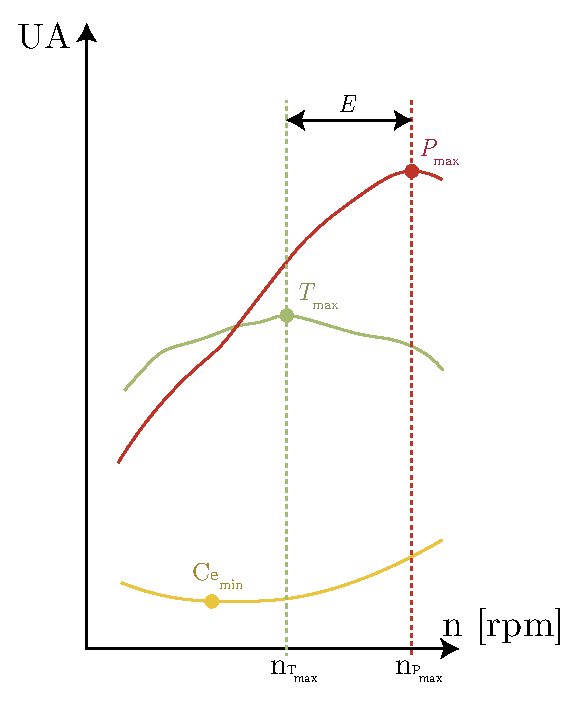
\includegraphics[width=.47\textwidth]{fig/curvaCaract.eps}
    \caption{Curvas características de un motor}
    \label{fig:curvacaract}
\end{figure}
\textbf{Consideraciones del ensayo.} Al realizar los ensayos para obtener los parámetros anteriores es muy importante tomar en cuenta las condiciones atmosfericas ya que $\etavol$ depende de estas y por lo tanto también la potencia. Se tiene que tomar en cuenta $p_{amb}$, $T_{amb}$ y en algunos casos humedad relativa $\phi_{amb}$.
\section{Disposición de cilindros}
Para motores de 4 tiempos ($720^\circ$ el ciclo completo) de $N$ cilindros se cálcula el ángulo por impulso: $\gamma_{imp} = \frac{720^\circ}{N}$


\begin{itemize}
    \item 
\end{itemize}

\section{Dispositivos de motor}
\subsection{Block de motor y otros elementos que lo acompañan}
\begin{itemize}
\item \textbf{Block de motor}
\begin{itemize}
\item Alberga cilindros/camisas
\item Puede tener sistema de refrigeración para refrigerar las paredes de los pistones 
\item Constituyes la estructura básica que soporta todos los componentes y demás elementos del motor
\item Debe ser rígido, permitir canalizaciones de aceite/liquido refrigerante,  parte superior totalmente plana para sellado contra culata
\end{itemize}
\item \textbf{Tapa de cilindros} o \textbf{Culata}
\begin{itemize}
\item Cierra la parte superior de los cilindros
\item Lleva orificios de refigeracion y conforma la parte superior de la cámara de combustión
\item Contiene el árbol de levas, bujías, inyectores, balancines y válvulas
\end{itemize}
\item \textbf{Junta de culata}
\begin{itemize}
\item Encargada de que la unión entre bloque y tapa sea estanca
\item Pueden ser de dos tipos, multilaminares/multimetalicas o convencionales de fibra
\item Para motores Diesel se necesita determinar la saliente sobre el bloque del pistón para elegir una junta
\end{itemize}
\item Bancadas o asientos de cigüeñal
\begin{itemize}
\item Donde apoyan los bujes de fricción que a su vez son el apoyo del cigüeñal del motor
\item Están recubiertos con un material más suave que el interior para atrapar metal o partículas disueltas en el lubricante
\end{itemize}
\item Semicárter
\item \textbf{Colectores de admisión}
\begin{itemize}
\item Su forma tiene gran influencia en el $\etavol$. Diferentes tipos de inyección como \textit{monopunto, multipunto.} Conduce gases del múltiple de admisión hacia la válvula de admisión
\end{itemize}
\item \textbf{Colector de escape}
\begin{itemize}
\item Conduce gases de escape hacia el silenciador de escape. Se suele hacer de fundición de hierro/acero inox. para soportar los grandes cambios de temperatura
\end{itemize}
\end{itemize}

\subsection{Lista de componentes del motor}
\begin{itemize}
\item \textbf{Cigüeñal}
\item Sistema de distribución
\begin{itemize}
\item Comprende todos los elementos necesarios para coordinar la apertura y cierre de válvulas con el giro del motor
\item El cigüeñal arrastra el \textbf{árbol de levas} que a su vez controla las \textbf{válvulas} que actuan a través de la \textbf{guía de válvulas}
\item Resortes o muelles de válvulas
\item Taques y balancines
\end{itemize}
\item \textbf{Volante de inercia}
\begin{itemize}
\item Está engranado porque está acoplado al piñón del burro de arranque que pone el motor en marcha
\item Suaviza el andar del motor
\end{itemize}
\item Conjunto \textbf{Pistón}
\begin{itemize}
\item Camisa
\item Perno o bulón de pistón
\item Biela
\item Émbolo
\item Cámara
\item Bujes de biela
\item Aros de pistón
\end{itemize}
\end{itemize}
\subsection{Cámaras de combustión}
\textbf{Tipo de cámara para motor Otto.} La cámara es conformada por la culata y el émbolo del pistón.
\begin{itemize}
\item \textbf{Cámara semiesférica.} La ideal. Diseño condicionado por la posición de las válvulas, difícil lograrlo
\item \textbf{Cámara hemisférica}. De característica parecida a la semiesférica. Válvulas posicionadas entre $20$-$60^\circ$
\item \textbf{Cámara tipo cuña.} Diseño mas antiguo con buena resistencia a la detonación y poca superficie interior
\item \textbf{Cámara de bañera.} De muy bajo rendimiento
\item \textbf{Cámara en el pistón.}  Se tiene una culata de superficie interior \textit{plana} por lo que el mismo hueco en el émbolo actúa de cámara. Muy buena homogeneización de la mezcla debido a la alta turbulencia adquirida por el fluido
\item \textbf{Cámara de inyección directa.} El émbolo del pistón posee deflectores que se concentre la mezcla rica en la cercanía a la bujía y pobre en su periferia
\end{itemize}

\textbf{Tipo de cámara para motor Diesel.}  El embolo suele tener una forma para favorecer la combustión.
\begin{itemize}
\item \textbf{Cámara de combustión directa.} La inyección se realiza directamente sobre el émbolo del pistón. Se usan inyectores de varios orificios. Bajo consumo especifico.
\item \textbf{Precámara o Cámara de combustión auxiliar.} Objetivo de provocar una gran turbulencia en el paso de la cámara auxiliar a la principal. Funcionamiento mas suave. Inyectores de un solo orificio. Se suele tener una bujía de precalentamiento. Hay dos tipos:
\begin{itemize}
\item Precámara de precombustión
\item Precámara de turbulencia
\end{itemize}
\end{itemize}

\subsection{Sistema distribución}
Se necesita que la relación de velocidades entre el árbol de levas y el cigueñal sea de $\frac{n_{cig}}{n_{arbLev}}=2$. El árbol de leva hoy en día se suele accionar por una correa. 

\textbf{Válvulas.} Partes de una válvula: Entalladuras (donde la sos tiene el resorte), Vástago, cabeza y el asiento cónico que apoya sobre el asiento de válvula de la culata. Pueden ir montadas \textit{en linea} (un solo arból de levas) o \textit{en doble linea} (permite mejor intercambio de gases) con un angulo de montaje de $20$-$60$\grad.

\textbf{Tipos de válvulas:}
\begin{itemize}
    \item Válvulas \textbf{monometálicas}
    \begin{itemize}
        \item Fabricadas de una pieza en bruto por moldeo por presión sin arranque de viruta
        \item Se somete la pinta del vástago a tratamiento posterior para endurecer y proteger químicamente
    \end{itemize}
    \item \textbf{Bimetálicas.} Dos materiales soldados por fricción. El vástago tiene baja fricción con la cabeza de material resistente a altas temperaturas
    \item Válvulas \textbf{refrigeradas con sodio}
    \begin{itemize}
        \item Válvula hueca que almacena sodio en su interior para aumentar la transferencia de calor aprovechando el movimiento alternativo de la válvula
        \item Reduce hasta en $100$\grad C la $T_{cabeza}$
\end{itemize}
\end{itemize}
    \textbf{La válvula de admisión suele tener un diámetro 20-30\% mayor.} \textbf{1.} Esto mejora la admisión de gases frescos que aumenta el $\etavol$. \textbf{2.} Además, durante el escape hay alta presión, lo que facilita su vaciado aun con poco diámetro. \textbf{3.} También por una cuestión de transferencia de calor, es deseable que sea de menor tamaño la válvula de escape para facilitar su enfriamiento.
    
    \textbf{Diámetros de cabeza de válvula.} $d_{admisi\acute{o}n}=b\cdot D$ con $b=0,40\hyph0,48$ donde $D$ es el diámetro del cilindro/embolo.
    
    \textbf{Alzada} $L$. Cuanto avanza la válvula para dejar los gases salir/entrar. $L/d=0,25\hyph0,30$

\textbf{Muelle de válvula.} Parece ser un \textit{resorte} pero es un \textit{muelle} (?) Actúa sobre la válvula para efectuar el cierre sobre el asiento y para que vuelva desde su máxima apertura (siempre comprimido). Se suelen usar muelles asimétricos para minimizar los efectos de inercia y vibraciones que puedan aparecer con un número alto de vueltas.   

\textbf{Árbol de levas.} Se requiere \textit{alta} precisión para fabricar el perfil de una leva. Se requiere un tratamiento superficial para evitar desgaste. Importante que esté lubricado el árbol.

El ángulo del cigüeñal que la válvula permanece abierta está dada por $\alpha_{abierta}=180^\circ +RCA+AAA$. El ángulo en el giro de árbol de levas es la mitad: $\beta=\frac{\alpha}{2}$.
\[
Dwell=\frac{\beta_{cierre}}{\beta_{cierre}+\beta_{abierto}}=\frac{\beta_{cierre}}{360^\circ}
\]
% Si alguien que no sabe \textbf{nada} en \textit{absoluto} de levas las tuviera que dividir en dos grupos:
%\footnote{Distinguir levas por su apariencia es imposible. Dos levas con función desplazamiento totalmente diferentes pueden parecer idénticas entre si y su aceleración ser muy diferente. Las levas son clasificada según su función de perfil.}
\begin{itemize}
    \item \textbf{Leva tangencial.} Movimiento rápido, picos de aceleración (por ende fuerzas inerciales mayores), permanencia mas grande. Desgaste infinito. \footnote{Una leva de perfil tangencial sufre por fatiga (desgaste por \textit{pitting}). Se necesita diseñar con un factor seguridad alto.}
    \item \textbf{Leva oval.} Velocidad nominal media, movimiento menor a la tangencial y permanencia menor. Desgaste bajo. Todas las levas se diseñan para reducir la aceleración y el desgaste. 
\end{itemize}

\textbf{Elementos de empuje.} Taqués, reguladores y varillas. Tienen gran superficie lo que disminuye el desgaste. Reparten esfuerzos laterales de mejor forma. Existen taqués hidráulicos que compensan dilataciones en el sistema de distribución (debido a cambio de temperaturas). 



\textbf{Elementos basculantes.} Balancines y palancas. Un balancín tiene un punto de giro cercano a su centro. Estos deben estar regulados para que cuando se dilate el sistema de distribución haya un dado juego de válvula entre la leva en su dwell y el taqué. Se puede lograr esto con placas calibradas sobre el taqué o ajustando el tornillo de regulación del balancín.

\subsection{Conjunto pistón}

\subsubsection{Camisa}
Tipos de camisa
\begin{itemize}
    \item Sin camisa. Se le dice \textbf{bloque integral} cuando el cilindro se elabora directamente en el mismo bloque de motor.
    \item \textbf{Camisa seca.} En contacto con el bloque de motor
    \item \textbf{Camisa húmeda.} En contacto con cámara de refrigeración del bloque de motor.
\end{itemize}


El émbolo del pistón está sujeto a fuerzas alternativas y consecuentemente apoya sobre la camisa (e el bloque integral).

\textbf{Desgaste por ovalamiento.} Se produce desgaste lateral por ovalamiento siendo mas importante en la parte que apoya el pistón cuando \textit{desciende} por ser mayores las fuerzas del gas sobre el émbolo que las fuerzas que se ejercen sobre el en el momento de ascenso.

\textbf{Desgaste cónico.} Se debe a que las fuerzas actuantes sobre el pistón son de mayor magnitud cerca del PMS que el PMI, lo que aumenta el desgaste en esa zona. 

\textit{Para minimizar dichos efectos se recurre al uso de camisa descentrado respecto el cigüeñal.}


\subsubsection{Fuerzas en el pistón}
Por cada ciclo del motor el pistón debe acelerar y frenar 4 veces. Esté movimiento alternativo somete el conjunto pistón a grandes esfuerzos alternativos.

El valor medio de la velocidad del pistón es:
\[
u_m = \frac{nL}{30} = \frac{\omega L}{\pi}
\]
donde $L$ es la carrera del émbolo, $n$ son las revoluciones del motor [rpm] y $\omega$ es la velocidad angular del motor [rad/s]. Resultado en [m/s].

Nos importa la relación carrera a diámetro $\frac{L}{D}$.

\begin{itemize}
    \item Carrera larga $\frac{L}{D}>1$
    \item Cuadrado $\frac{L}{D}=1$
    \item Supercuadrado $\frac{L}{D}<1$
\end{itemize}

{\bf La detonación.}
Se desea evitarla a todos costo. Sucede cuando una mezcla fresca explota antes que la alcance el frente de llama de la mezcla encendida(ignición controlada). Se puede evitar la detonación mediante el avance de encendido. Cabe destacar que si la mezcla se enciende antes de la chispa deja de ser detonación y pasa a ser llamado \textit{pre-ignición} o \textit{autoencendido}. En este ultimo proceso \textbf{no} participa la chispa del encendido. 




\vspace{.9cm}
{\centering 
{\bf \LARGE Segundo Parcial \par}
}
\begin{center}
\vspace{-.2cm}\rule{3cm}{2pt}\par
\vspace{-.2cm}
\end{center}

\section{Dosificación Aire--Combustible}
\begin{itemize}
    \item Sistema de Carburador
    \item Sistema Inyección
    \begin{itemize}
        \item Gestión Mecánica
        \item Gestión Electrónica (Actualidad)
        \begin{itemize}
            \item Directa
            \item Indirecta
        \end{itemize}
    \end{itemize}
\end{itemize}
\subsection*{Carburador}
Trabaja con mezcla levemente rica con el principio de Bernoulli. En ralentí la mariposa está cerrada por lo que el grado de depresión es muy bajo. Al carburador le cuesta tomar combustible y la pulverización es muy baja. Para suplir esto están los circuitos de ralentí.
\begin{itemize}
    \item Dispositivo de cebado automático
    \item Bomba de aceleración
\end{itemize}


\subsection{Sistemas de inyección}
Se tienen tres subsistemas:
\begin{itemize}
    \item Sensores: Traducen una magnitud física en pulsos digitales/diferencial de potencial/corriente. La medida física suele ser denominada como {\it variable de funcionamiento del motor.}
    \item ECU: Engine control unit. Computadora. Compara los datos de los sensores con su mapeo y en base a esto le da ordenes a los actuadores
    \item Actuadores. Elementos eléctricos y/o electrónicos que ejecutan órdenes.
\end{itemize}
{\bf Componentes básicos}
\begin{itemize}
    \item Sensores
\begin{itemize}
    \item Sensor de masa de aire. Mass Air Flow (MAF). Anemometro (hot wire sensor).
    \item Sensor de depresión. Manifold Absolute Pressure (MAP).
    \item Sensor de apertura de válvula aceleradora (mariposa)
    \item Sensor de pedal
    \item Sensor de detonación.
    \begin{itemize}
        \item Por vibraciones
        \item Por revoluciones. La detonación frena brevemente el pistón para luego acelerarlo.
    \end{itemize}
    \item Sensor de temperatura de aire.
    \item Sensor de RPM
    \begin{itemize}
        \item Efecto Hall. La interacción de la corriente en un entorno conductivo con un campo magnético externo hace aparecer un diferencial de potencial.
        \item Inductivo. Bobina, imán y rueda dentada. El eje de la bobina se alinea con la rueda dentada y se altera el campo magnético creando así una señal de corriente alterna (CA).
    \end{itemize}
    \item Sensor de fase
    \item Throttle position sensor
    \item Sonda Lambda (sensor de oxigeno)
\end{itemize}
    \item Actuadores
    \begin{itemize}
   \item Valvula EGR (Exhaust Gas recirculation): Se re-introducen gases de escape al múltiple de admisión, lo cual no aporta oxigeno para la combustión. Esto hace caer la temperatura en la cámara de combustión y se reduce la formación de $NO_x$
   \item Bobina de encendido
   \item Inyectores
   \item Valvula de purga del Canister
   \item Comando de la válvula aceleradora
   \item Lampara de advertencia de fallas
   \item Bomba de combustible
   \end{itemize}
   \item Otros componentes relacionados
   \begin{itemize}
          \item Canister: Receptáculo que tiene carbón activado. Cuando hay mucha presión en el deposito de combustible absorbe los vapores y luego los libera cuando se produce una depresión en el múltiple de admisión.
          \item Catalizador
   \end{itemize}
\end{itemize}

\textbf{Pregunta}: Como es la conexión (a multimetro) para verificar el funcionamiento de los siguientes sensores: Sonda Lambda 4 cables, Sensor de temperatura, sensor MAP.
%%%%%%%%%%%%%%%%
%% FIN DE LISTA
%%%%%%%%%%%%%%%%
{\bf Diferencias respecto al carburador}

\begin{itemize}
    \item Menor condensación en múltiple de admisión
    \item Respuesta más rápida (combustible más cercano a la cámara de combustión)
    \item Menor contaminación
    \begin{itemize}
        \item Uso de catalizador para convertir $NO_x$, $CO$ y $H_xC_y$ en gases no nocivos.
        \item Control preciso del tiempo de inyección con mapeo de tiempo ideal para inyectar combustible
        \item Recirculación de gases de escape, disminuye $NO_x$
        \item La mejora en la respuesta resulta en un ralentí más parejo y menor condensación de vapor de combustible en múltiple de admisión
    \end{itemize}
    \item Menor consumo de combustible
    \begin{itemize}
        \item Uniformidad de la mezcla en cada cilindro
        \item Mejor atomización del combustible, mejora $\eta$.
        \item La localización del inyector provoca menor licuefacción de combustible
        \item Corte de combustible en desaceleración
    \end{itemize}
    
\end{itemize}

{\bf Cálculo de aire de entrada} Se puede calcular con sensores tipo: \emph{RPM, volumétrico/paleta(VAF), sensor ultrasónico Von Karman, depresión en ele múltiple de admisión, hilo caliente}.

{\bf La central de control (ECU)} está compuesta por: \emph{Unidad de salida, microprocesador, memoria EPROM y RAM, sistema auto-diagnostico, conexión con sistema CAN.} Las señales de los sensores son contrastadas con los datos escritos en la base de datos (mapas) y a partir de esto se efectúan parámetros de acción para los actuadores.

{\bf CAN.} Controller Area Network. En su forma más simple, conecta todos los electrónicos del auto juntos permitiendo la comunicación libre entre ellos.

{\bf Sistemas de gestion de motor.} Central de control que gestiona no solo la inyección pero también el encendido. LA relación entre gases nocivos emitidos y el control eficiente de un motor es \emph{estrecha.}

{\bf Clasificación por cantidad (o ubicación) de inyector}

\begin{itemize}
    \item Sistemas monopunto (indirecta): inyector único para todos los cilidros o por bancada.
    \item Multipunto: Existen tantos inyectores como cilindros tiene el motor.
    \begin{itemize}
        \item Puede ser \textbf{directa} o \textbf{indirecta}(afuera de los cilindros)
    \end{itemize}
\end{itemize}

{\bf Clasificación por secuencia de inyección}

\begin{itemize}
    \item Simultanea. No respeta el mejor momento para inyectar combustible (antigua)
    \item Grupal. Entremedio entre simultanea y secuencial
    \item Secuencial. Se hace la inyección en el momento indicado para cada cilindro
\end{itemize}

{\bf Mezcla estequiométrica.} Se logra con {\bf14,7} gr de aire por cada 1 gr de gasolina. {\bf 14,5} gr de aire para cada 1 gr de Diesel. Para gases es mayor, estando entre 15,8:1 (propano) y 17,4:1 (metano al 97\%).

{\bf Gases de escape}

\begin{itemize}
    \item $CO$. Altamente tóxico al humano. Valores altos indican una mezcla rica o una combustión incompleta
    \item $NO_x$. Al reaccionar con rayos ultravioletas genera ácido nítrico (smog). Se forma en condiciones de altas temperaturas. Depende en gran medida del adelanto de encendido. Para un $\lambda\approx 1,07$ se tiene un pico de $NO_x$ producido
    \item $H_xC_y$. (hidrocarburos). Contamina suelo. Formado por mezcla rica, mala combustión durante mezcla pobre o escape contaminado con aceite
    \item $CO_2$. Absorbe radiación infrarroja y por ende contribuye al efecto invernadero. Se desea que todo el carbón de los hidrocarburos se convierta en $CO_2$. En el catalizador se trata de oxidar $CO$ remanente $\rightarrow$ $CO_2$. Niveles bajos indican una combustión mala o problemas de encendido.
    \item $O_2$. Alto porcentaje de $O_2$ indica una mezcla pobre, escape roto, combustión incompleta o desgaste del catalizador
    \item $SO_2$. Nocivo para el medio ambiente, genera lluvia ácida. No se encuentra en grandes concentraciones en motores a gasolina. $SO_2$ más común en Diesel
\end{itemize}

{\bf Formas para controlar emisiones}

\begin{itemize}
    \item Disminución de relación de compresión. Temperatura $T\downarrow \quad$ $NO_x\downarrow$ 
    \item Aumento de ángulo de cruce de válvulas. $\eta_{vol}\uparrow$. Concentración aire fresco $\uparrow \Rightarrow $ $H_xC_y \downarrow$
    \item Cámaras hemisféricas, aumento de número de válvulas $\uparrow \eta_{vol}$
\end{itemize}

\begin{figure}[!htb]
    \centering
    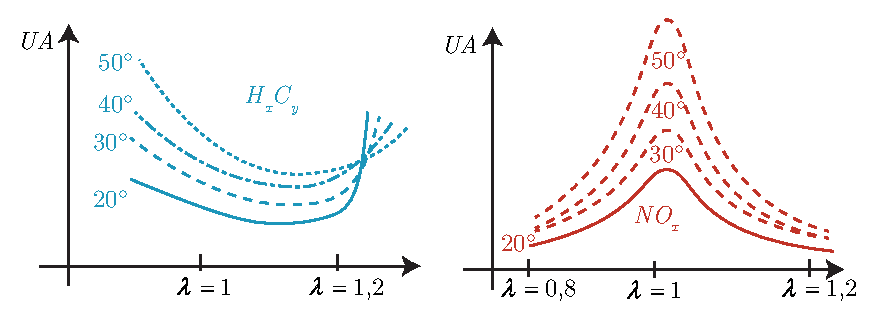
\includegraphics[width=.47\textwidth]{fig/aperturaEscapeGases.eps}
    \caption{Efecto de apertura de escape (AE) sobre los gases de escape producidos. La producción de $CO$ aumenta a mezclas más ricas ($\lambda<1$) con el aumento del AE.}
    \label{fig:aperturaEscape}
\end{figure}
\subsection[Sonda Lambda]{Sonda $\lambda$}
La sonda lambda mide la \textit{proporción} de $O_2$ presente en una mezcla de gases.
\[
\lambda = \frac{\textrm{Proporción de $O_2$ medida}}{\textrm{Proporción de $O_2$ teórica}}
\]

El valor $\lambda$ es la razón entre la proporción oxigeno presente en los gases de escape y la proporción de oxigeno teórica que debería estar presente después de una combustión estequiométrica.

{\color{magenta}La sonda $\lambda$ no mide el oxigeno de la mezcla antes de la combustión, está ubicada en el escape!} Cuando $\lambda =1$ se tiene una mezcla estereométrico, llamada la \emph{Zona Lambda}. Si $\lambda<1$ se dice que se tiene una mezcla rica (en combustible) y vice versa. 

Se suele trabajar con dos sondas cuando se quiere verificar el correcto funcionamiento del catalizador, la sonda lambda primaria (antes del catalizador) y la sonda lambda secundaria (después del catalizador). Comparando las lecturas de ambas se debería ver una disminución del oxigeno (porque hay oxidación ocurriendo en el catalizador!).

El motor puede trabajar en ``Lazo abierto'' o ``Lazo cerrado'' en conjunto con la Sonda Lambda. 

{\bf Lazo cerrado.} El motor busca reducir contaminación disminuyendo o aumentando tiempo de inyección según la lectura de la Sonda Lambda. En este régimen la señal oscila entre $100$mV y $900$mV,

{\bf Lazo abierto.} En ciertas situaciones no es posible trabajar con valores de mezcla estequiométricas. Si se tiene un motor en frío, o en aceleración brusca la central de control no ajusta la mezcla con valores estequiométricos, funcionamiento denominado \emph{lazo abierto}.

\begin{figure}[!htb]
    \centering
    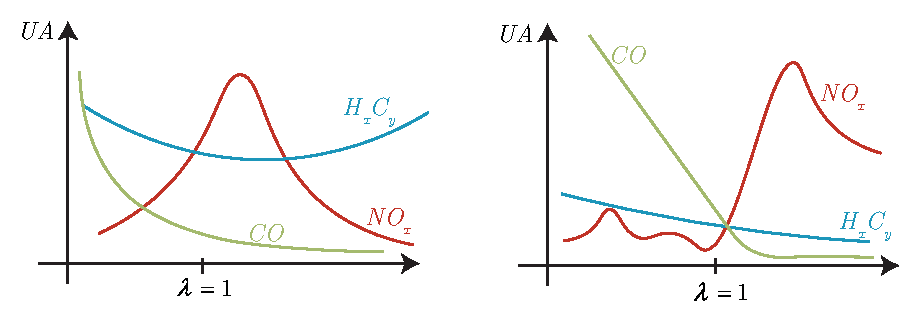
\includegraphics[width=.47\textwidth]{fig/lambdaEscape.eps}
    \caption{Medición sonda $\lambda$ antes y después del catalizador. La curva del $CO_2$ antes del catalizador es idéntica al \NX{} pero con el pico en $\lambda=1$}
    \label{fig:lambdaCatalizador}
\end{figure}

{\bf Catalizador}

Idealmente hace reaccionar todos los gases nocivos, efectivamente neutralizando la huella ambiental \emph{casi} por completo. 

Funciona a $400-700 ^\circ C$ con una mezcla del alrededor de $\lambda =1$ para lograr maximizar su efectividad. Se busca oxidar: $2CO+O_2\rightarrow 2CO_2$, $H_xC_y+(\frac{x}{4}+y) O_2\rightarrow \frac{x}{2} H_2O+y CO_2$ (reacciónes exotérmicas)  y reducir los óxidos del nitrógeno $2NO_x\rightarrow N_2+xO_2$. Se espera que a la salida del catalizador la lectura de la sonda lambda secundaria sea menor a la primaria
\subsection{Control de mezcla}
\begin{itemize}
    \item \textbf{Cut-off}. Cuando hay un cierre abrupto de la mariposa (se suelta el pedal de aceleración a RPM altas) se advierte al ECU. La ECU corta el suministro de combustible y fija el AE para evitar la formación de \HC
  
    \item \textbf{Ralentí}. Al número mínimo de revoluciones se inyecta pequeñas cantidades de combustible para permanecer en funcionamiento
    \item \textbf{Dash Pot} o \textbf{retardo de cierre de mariposa}. Impide el cierre total de la mariposa para prevenir la formación de \HC
\end{itemize}
\subsection{Válvula EGR}
Recirculación de gases de combustión que enfrían la cámara reduciendo así la cantidad de \NX producido. Disminuye la potencia, la eficacia del lubricante (introduce material particulado). La válvula EGR no actúa en ralentí, \NX, motor frío o baja carga.

{\bf Eliminación de gases de cárter de motor.}
$CO$ en bajas proporciones y \HC en altas proporciones. Originan de evaporación de compuestos de aceite y restos de combustible y gases de combustión que se escapan de la cámara a través de los aros del pistón. Conlleva con una \emph{perdida de potencia, aparición de incrustaciones en trayecto admisión--cámara}.

{\bf Vapores de tanque de combustible.} 
Se almacenan los vapores formados en el tanque adentro de un canister de carbón activado que son alimentados a la cámara por medio de una electroválvula.

{\bf Inyección de aire.}
Se puede inyectar aire al trayecto después de la válvula de escape para realizar una post-combustión del $CO$ y \HC para aliviar la tarea del catalizador.

{\bf Bomba de combustible.}
La bomba de combustible tiene el trabajo de presurizar el combustible para la inyección.

{\bf Regulador de presión de combustible.}
Se trata de mantener la diferencia de presión entre el combustible y el múltiple de admisión siempre igual. Estudiar las diferentes posiciones posibles del regulador (con retorno/sin retorno/demanda controlada)

{\bf Atenuador de pulsaciones.}
Amortigua pulsaciones en el fluido de la rampa de inyectores mediante un resorte.


\subsection{Actuadores}

{\bf Inyectores.}
Electrovalvulas 

{\bf Bomba lineal.}
La cantidad de elementos de bombeo es igual al número de cilindros en el motor y se situan en linea. 

Esta hecha de los siguientes elementos 

\begin{itemize}
    \item La bomba (generador de presión)
    \item El regulador mecánico (regula RPM según régimen)
    \item El variador de avance (ajusta el comienzo de inyección en función del número de revoluciones)
    \item Arbol de levas
\end{itemize}

Conocer bien la función de los reguladores mecánicos.

\subsection{Diesel bomba EDC}
Bomba aspira combustible, lo presuriza hasta la presión de inyección.

El combustible pasa a través de una bomba de transferencia rotativa que alimenta la cámara de compresión de émbolos radiales \emph{cuando la electroválvula se abre}.

Cuando la electroválvula se cierra, el combustible de la cámara de compresión se dirige al inyector correspondiente. Una vez que termina la inyección la electroválvula se abre y cae la presión nuevamente.

{\bf Avance de inyección.} 
Se realiza mediante la acción del embolo del corrector sobre el embolo de control

\subsection{Common Rail}
Controla la inyección de combustible Diesel en el momento correcto, con el caudal correcto y con la presión necesaria. Se reduce el ruido y favorece el motor.

Se compone de:
\begin{itemize}
    \item Unidad de control
\item Bomba de alta presión
\begin{itemize}
    \item Válvula de desconexión del elemento
    \item Válvula reguladora de presión
    \item Previo a la entrada de la bomba: Filtro de combustible y bomba previa
\end{itemize}
\item Acumulador de alta presión (Rail)
\begin{itemize}
    \item Sensor de presión Rail
\end{itemize}
\item Inyectores
\item Medidor de masa de aire
\item Sensor de revoluciones de cigüeñal
\item Sensor de temperatura del líquido refrigerante
\item Filtro de combustible
\item Sensor del pedal del acelerador
\item Turbocompresor
\end{itemize}

{\bf Diferencias con inyectores convencionales}
\begin{itemize}
    \item Presión constante después de un cierto número de vueltas (convencionales aumenta linealmente)
    \item Presión de inyección constante durante inyección. Las combustiones favorables requieren pequeños caudales al comienzo de la inyección. Por eso el sistema Common Rail cuenta con una inyección previa pequeña ($1-4\si{mm^2}$)
\end{itemize}

{\bf Características de la inyección previa.}
Puede estar adelantada del PMS hasta $90^\circ$ aunque antes de los $40^\circ$ esto puede ocasionar problemas al tener contacto entre el combustible y las paredes del cilindro y pistón, provocando una dilución inadmisible del aceite lubricante.

Con la inyección previa se logra que \emph{la presión de compresión aumente ligeramente mediante una combustión parcial previa al PMS, reducir el retardo de encendido a la inyección principal, reducir el aumento de la presión de combustión y suavizar los picos de presión.}

{\bf Características de la inyección posterior.}
Se puede aplicar por los efectos reductores de los aditivos del combustible. Puede suceder hasta $200^\circ$ después del cigüeñal durante la etapa de expansión o escape.

\subsection{Combustible}
{\bf Reacciones.}
Recordemos que el aire es una mezcla de varios gases. En su mayor parte es Nitrogeno (78,09\%), oxigeno (20,95\%) y argon (0,93\%). $\frac{78,09}{20,95}=3,73$  
La reacción general para aire en exceso:
\begin{align*}
C_m H_n O_p+Y O_2+&3,73Y(N_2)\longrightarrow \\ mCO_2 +\tfrac{n}{2}& H_2O +3,73 Y (N_2)+(Y-Y_{cc})O_2
\end{align*}
donde $Y$ es la cantidad de moles de oxigeno suministrados. $Y_{cc}$ es la cantidad de moles de oxigeno requeridos para lograr la reacción estequiométrica.

En el caso que $Y=Y_{cc}$ entonces se tiene una mezcla estequiometrica y no se produce $O_2$.

La reacción general para mezcla rica:
\begin{align*}
C_mH_nO_p+&YO_2+3,73YN_2\longrightarrow \\ &XCO+(m-X)CO_2+\tfrac{n}{2}H_2O+3,73YN_2
\end{align*}
\begin{align*}
\frac{p}{2}+Y=\frac{X}{2}+&(m-X)+\frac{n}{4}\\
&\Rightarrow X=2\left(m+\frac{n}{4}-\frac{p}{2}-Y \right)=2(Y_{cc}-Y)
\end{align*}
la formula queda 

\begin{align*}
C_mH_nO_p + YO_2+3&,73YN_2\longrightarrow \\  2(Y_{cc}-Y)CO+2(&Y -Y_{min})CO_2+\tfrac{n}{2}H_2O+3,73YN_2
\end{align*}

{\bf Hidrocarburos liquidos.}
\begin{itemize}
\item Bencinas o Gasolina=nafta. Motores encendidos por chispa.
\item Gasóleos: Gasoil, fuel oil etc.
\item Kerosene. Alto poder calorifico. No se suele usar por su alta viscosidad y contaminación.
\item Benzol y alcoholes. Considerados carburantes
\end{itemize}

{\bf Poder antidetonante o número de octano (NO).}
Se obtiene comparando el carburante con combustibles de referencia: el \emph{iso-octano} y el \emph{heptano}\footnote{Antiguamente iso-octano y tetraetil de plomo.}
Iso-octano tiene cualidades muy antidetonantes y se lo toma como referencia $NO=100$. El Heptano en cambio detona con facilidad $NO=0$.

Un combustible que a la misma relación de compresión que una mezcla 80\% de iso-octano y 20\% heptano, tiene un $NO=80$.

{\bf Formas de medir el} $NO$.
\begin{itemize}
    \item $RON$ Research Octane Number: Asociado al funcionamiento con altas velocidades y detonación media o suave
    \item $MON$ Motor Octane Number: Asociado a velocidades altas, temperaturas y funcionamiento a media o alta carga.
\end{itemize}

\section{Lubricantes}
Tres tipos básicos de lubricación. Hidrodinámico o fluido, rozamiento semifluido, rozamiento seco. Lo ideal es llegar a lubricar hidrodinámico (no hay contacto entre partes solidas).

{\bf Funciones y algunas propiedades necesarias del aceite lubricante:}%iento lo máximo posible ento lo máximo posible
\begin{itemize}
\item Refrigerar zonas a lubricar. Refrigerar zona interior del pistón.
\item Aumentar estanqueidad entre segmentos y el cilindro elevando la compresión
\item Amortigua las cargas fluctuantes sobre cojinetes
\item Limpia y transporta carbonilla y partículas al filtro.
\item \textbf{Protege contra la corrosión.} Previene formación de ácidos que carcomen la parte más frágil del motor: bujes de apoyo del cigüeñal y árbol de levas.
\item Se lo aditiva así mantiene la viscosidad en caliente y la fluidez en frío. Hoy en día TODOS los aceites tienen aditivos.
\begin{itemize}
    \item \textbf{Detergente.} Limpia partes mecanicas
    \item \textbf{Dispersante.} ``Rodea" particulas sueltas y evita formación de compuestos
    \item \textbf{Antiespumante.} Evita formación de burbujas para no disminuir capacidad lubricante
\end{itemize}
\item El aceite que pasa a la cámara tiene que quemarse sin dejar residuos
\item Untuoso: Capacidad de adherirse a las superficies metálicas
\item 
\end{itemize}

\subsection{Parámetros característicos de un lubricante.}
Las escalas de SAE se usan para medir la viscosidad de un aceite.
{\bf Índice de viscosidad.}
El \emph{viscosity index} o $VI$ nos dice cuanto varía la viscosidad ante un cambio de temperatura.
\[
\frac{\di \mu}{\di T}\propto VI^{-1}
\]
osea que la viscosidad de un lubricante con alto $VI$ no varía fuertemente con cambios de temperatura.

Un aceite \textbf{multigrado}, a diferencia de un aceite monogrado tiene mayor margen de temperatura de trabajo (alto $VI$). Esto se logra con aditivos. SAE los denomina con una ``W". Un \textit{SAE 20W 40} se comporta como un \textit{SAE 20} a bajas temperaturas y como un \textit{SAE 40} a altas temperaturas.

{\bf Total Base Number (TBN).}
La propiedad \textit{detergente} de los aceites. Gracias a esta propiedad los aceites mantienen en suspensión las partículas, evitando que entren en contacto con superficies e incrustaciones.

Los aditivos que logran esta mejora (\textbf{TBN}) son químicamente \textit{básicos}. De está forma contrarrestan también la formación de ácido sulfúrico ($H_2SO_4$) por causa del contenido de azufre en el combustible. Suele pasar con Diesel por el alto contenido de azufre.

{\bf Clasificación API.}
Usada en EE.UU y la mayor parte de latinoamerica.\footnote{En europa el organismo de control es la ACEA}. Las categorías API se dividen en dos series:
\begin{itemize}
\item S - Spark ignition (motores Otto)
\item C - Compression (motores Diesel)
\end{itemize}
El número que procede a las letras de categoría es el tiempo del motor (dos tiempos/cuatro tiempos).
 
Si se indica que es ``Plus'' es porque cumple con las especificaciones de la categoría indicada y los \textit{excede!} Esto no significa que cumple con las especificaciones de la próxima categoría!

\textbf{El API Doughnut}
Un ejemplo de una clasificación API: \texttt{API SERVICE CI-4/SL} Nos dice que es un aceite para motores Diesel de \textbf{4} tiempos con la posibilidad de usarse con motores de Otto calificados para \textbf{SL}. (C=Compression Ignition, S=Spark Ignition). La clasificación del aceite es \textbf{SL}, una clasificación anterior a  \textbf{SN} aún no obsoleta.
\begin{figure}[htb!]
    \centering
    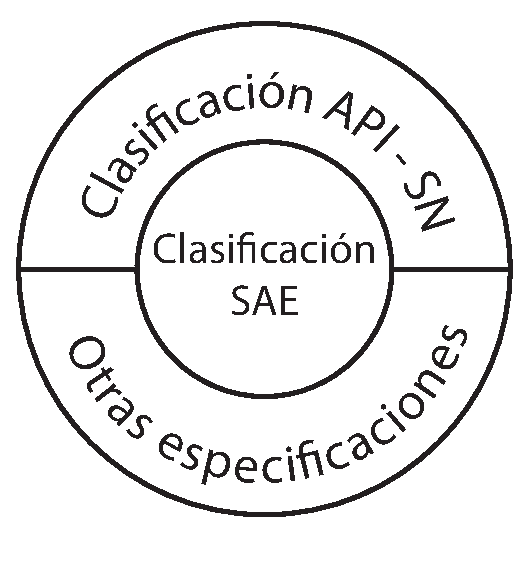
\includegraphics[width=.25\textwidth]{fig/api.eps}
    \caption{Como ubicarse con un API ``doughnut". Las últimas letras son \emph{SN}, la clasificación del aceite, en este caso para motor Otto. En el momento que fue escrito este documento la última clasificación del API era la SN Plus para motores Otto aprobada el 9 de noviembre 2017 y CK-4 para motores Diesel aprobada 2017. Existe la clasificación FA-4 para motores Diesel de bajo contenido de sulfuro ($<$0,0015\%), introducida 2017.}
    \label{fig:APIclasification}
\end{figure}

\subsection{Sistema de lubricación del motor endotérmico}
\begin{itemize}
    \item Engrase a presión (el más utilizado). Típica presión de engrase: 0,5-1 bar a ralentí. 3-5 bar en régimen
    \item Engrase por mezcla con el combustible
\end{itemize}

{\bf Engrase a presión.} El aceite pasa por los canales del block y la culata, lubrica los cojinetes, rebalsa y cae al cárter. En el cárter es succionado por la bomba haciéndolo pasar por un filtro y al conducto principal y se repite. A la salida de la bomba hay una válvula de descarga que limita la presión máxima del aceite.

Los apoyosLos componentes engrasados a presión 

\textbf{Filtro.} Cuando está puesto en \textit{serie} todo el aceite pasa por el filtro. Menos común son los filtros de \textit{derivación} que solo filtran el aceite del cárter. Como regla general se suele cambiar el filtro cada 15000 km o al año.
}
\end{document}